\chapter{Vyhľadávacie stromy: \vb{<set>} a \vb{<map>} v STL}
\label{sect:stromy}

Pri farbení Mandelbrotovej množiny v závere minulej kapitoly som robil túto vec:
''{\em \ldots pre každý počet iterácií } [som] {\em našiel maximálnu a minimálnu hodnotu
\ldots}''. Ak si sa pozrel do môjho programu, tak si videl, že som trochu cheatoval
a použil som typ \prg!map! z STL, o ktorom som ti doteraz nehovoril. Ale v tejto
kapitole to chcem napraviť. Začnime jednoduchou rozcvičkou:

\begin{uloha}
  Na vstupe je číslo $n$. A potom postupnosť príkazov. Každý príkaz je tvaru
  \vb{! x} alebo \vb{? x} a posledný príkaz je \vb{\#}. 
  Predpokladajme, že máme $n$ žiaroviek očíslovaných $1,\ldots,n$, 
  ktoré su na začiatku vypnuté. Príkaz \vb{! x} znamená, že sme prepli žiarovku
  číslo $x$ (ak bola vypnutá, bude zapnutá a naopak). Pre každý príkaz \vb{? x}
  treba vypísať, \vb{svieti} alebo \vb{nesvieti} podľa toho, v akom stave je práve žiarovka
  číslo $x$.
\end{uloha}

Jednou z možností, ako túto úlohu vyriešiť, bolo urobiť si vektor $n$ hodnôt typu \prg!bool!
tak, že v \prg!a[i]! si budeme udržiavať stav $i$-tej
žiarovky. Predpokladajme teraz ale, že by žiarovky neboli očíslované $1$ až $n$, ale
že by mali iba výrobné čísla. Vstup by mohol vyzerať napríklad:\\

\begin{outputBox}
! 3736272
! 843984
? 3736272
! 84872634
! 72876
? 99
? 843984
#
\end{outputBox}

Problém je, že nevieme, aké výrobné čísla sa na vstupe objavia. Nemôžme si držať v pamäti 
pole pre všetky možné čísla, takže chceme mať zapamätané iba tie žiarovky, ktoré sme 
už videli. Teraz ale stoja proti sebe dve veci: ak chcem nájsť stav žiarovky s číslom 
\vb{id}, hodilo by sa mi mať žiarovky utriedené podľa čísla: mohol by som použiť
binárne vyhľadávanie, aby som zistil, či \vb{id} svieti. Ak ich utriedené nemám,
musím zakaždým prejsť všetky, čo trvá dlho. Na druhej strane, keď sa  objaví nová
žiarovka, ľahko ju pridám na koniec, ale potom nebudú utriedené. Musel by som 
všetky žiarovky v poli poposúvať, čo zase trvá dlho. 
Riešenie je namiesto poľa (vektora) použiť dátovú štruktúru, ktorá nemá všetky dáta
v jednom kuse pamäte, ale vo viacerých, ktoré na seba navzájom ukazujú pointrami. Tým
sa bude dať docieliť, že pri vkladaní nového prvku
bude namiesto posúvania všetkých hodnôt stačiť presmerovať
zopár pointrov. 

 Aby som ti ukázal, ako také štruktúry fungujú, začnime s jednoduchším príkladom
a k žiarovkám sa vrátime na konci kapitoly.

\begin{uloha}
  Úradník má kartotéku, kde má uložené spisy očíslované $0,1,\ldots,n-1$ (na začiatku
  v tomto poradí).
  Keď potrebuje nájsť spis $i$, začne prehľadávať zaradom od začiatku kartotéky
  a vždy prečíta číslo spisu, až kým nenájde ten s číslom $i$. Ten potom použije a 
  uloží na začiatok kartotéky. Napíš program, ktorý má na vstupe čísla $n, m$ a potom
  $m$ čísel spisov (medzi 0 a $n-1$). Pre každé číslo spisu vypíš riadok, v ktorom 
  sú čísla spisov, ktoré úradník prečítal pri hľadaní. Napríklad

  
  \begin{column}{0.45}
  \begin{outputBox}
6 4
5
3
4
1
\end{outputBox}
\end{column}
\begin{column}{0.45}
\begin{outputBox}
0 1 2 3 4 nasiel som 5!
5 0 1 2 nasiel som 3!
3 5 0 1 2 nasiel som 4!
4 3 5 0 nasiel som 1!

\end{outputBox}
\end{column}
\end{uloha}


Na riešenie použijeme dátovú štruktúru {\em spájaný zoznam} ({\em linked list}).\indexItem{Alg}{spájaný zoznam}
Každý prvok zoznamu je uložený v samostatne alokovanej pamäti a má pointer
na nasledujúci prvok. Spravíme si typ

\begin{lstlisting}
struct Node {
  int val;
  Node *nxt;
  Node(int _val = -1, Node *_nxt = nullptr) {
    val = _val;
    nxt = _nxt;
  }
};
\end{lstlisting}

v ktorom bude jeden prvok zoznamu\footnote{%
  Možno ťa zaskočilo, že súčasťou typu \vb{Node} je premenná \vb{nxt}, ktorá
  je pointer na typ \vb{Node}. Nie je v tom ale nič zvláštne -- pointer je iba číslo
  adresy v pamäti. Typ pointra (v našom prípade \vb{Node *}) iba hovorí kompilátoru,
  že na adrese uloženej v premennej \vb{nxt} má očakávať premennú typu \vb{Node}.
  Pretože všetky pointre sú rovnako dlhé, kompilátoru nevadí, že typ \vb{Node} zatiaľ nie 
  je pripravený, stačí mu vedieť, koľko miesta treba v pamäti vyhradzovať.
  }. V programe budeme mať zoznam zapamätaný iba pointrom
na jeho začiatok \prg!Node *head;! Zoznam \vb{[0 1 2 3 4 5]} by v pamäti vyzeral takto:\\
    

    \def\llnode(#1,#2)[#3]#4{
      \begin{scope}[shift={(#1,#2)}]
        \draw [\nodecolor, rounded corners=2pt] (-0.5,-0.5) rectangle (0.5,0.5)
        (-0.5,0) -- (0.5,0)
        (-0.5,0.25) node [anchor=west]{{\robotomono val:}}
        (0.3,0.25) node[anchor=center]{{\robotomono #4}}
        (-0.5,-0.25) node [anchor=west]{{\robotomono nxt:}}
        (0.3,-0.25) node[anchor=center] {$\bullet$};
        \coordinate (n#3) at (0.3,-0.25);
        \coordinate (b#3) at (-0.5,0.25);
      \end{scope}
    }

    \def\head(#1,#2){
      \node[\nodecolor,anchor=east] (head) at (#1,#2) {\vb{head:}};
      \node[\nodecolor,right = 0mm of head, ] (headbullet) {$\bullet$};
    }


%\tikzset{external/force remake}
\centerline{
  \begin{tikzpicture}[xscale=1.4*0.8,yscale=0.8]
    {\small
    \def\nodecolor{cyan!50!blue}
    \foreach \v/\c[count =\i] in {0/A, 1/B, 2/C, 3/D, 4/E, 5/F} {
      \llnode(1.5*\i,0.5)[\c]{\v}
    }
    \foreach \x/\y in {A/B, B/C, C/D, D/E, E/F} {
    \draw[->,\nodecolor,shorten >= 0.15ex](n\x) to[out=0, in=180] (b\y);
    }
    \head(0,0);
    \draw[\nodecolor,->, shorten >= 0.15ex] (headbullet) to[out=0,in=180] (bA);
    \draw[\nodecolor,-|] (nF) to [out=0,in=90] ++(0.5,-0.5);
    }
  \end{tikzpicture}
}



Vyrobíme ho jednoducho:

\begin{lstlisting}
head = nullptr;
for (int i = 0; i < n; i++)
  head = new Node(n - 1 - i, head);
\end{lstlisting}

V cykle vždy pri vyhodnocovaní pravej strany priradenia 
vyrobíme novú premennú typu \vb{Node}, v ktorej nastavíme \vb{val}
na správnu hodnotu a \vb{nxt} na rovnaké miesto, ako práve ukazuje \vb{head}.
V priradení potom nastavíme \vb{head}, aby ukazoval na túto novú premennú.\\


\centerline{

  \begin{tikzpicture}[xscale=1.4*0.8, yscale=0.8]
    {\small
    \def\nodecolor{cyan!50!blue}
    \foreach \v/\c[count =\i] in {4/A, 5/B} {
      \llnode(0.8+1.5*\i,0.5)[\c]{\v}
    }
    \foreach \x/\y in {A/B} {
    \draw[->,\nodecolor,shorten >= 0.15ex](n\x) to[out=0, in=180] (b\y);
    }
    \head(0,0);
    \draw[\nodecolor,->, shorten >= 0.15ex] (headbullet) to[out=0,in=180] (bA);
    \draw[\nodecolor,-|] (nB) to [out=0,in=90] ++(0.5,-0.5);
    
    \def\nodecolor{orange!80!black}
    \llnode(0.5,1.2)[C]{3}
    \draw[\nodecolor,->, shorten >= 0.15ex] (nC) to [out=0,in=90] ($(bA)+(0.5,0.25)$);
    }  
  \end{tikzpicture}
  \hfill
  \begin{tikzpicture}[xscale=1.4*0.8,yscale=0.8]
    {\small
    \def\nodecolor{cyan!50!blue}
    \foreach \v/\c[count =\i] in {4/A, 5/B} {
      \llnode(1.5+1.5*\i,0.5)[\c]{\v}
    }
    \foreach \x/\y in {A/B} {
    \draw[->,\nodecolor,shorten >= 0.15ex](n\x) to[out=0, in=180] (b\y);
    }
    \head(0,0);
    
    \llnode(1.5,1.2)[C]{3}
    \draw[\nodecolor,->, shorten >= 0.15ex] (nC) to [out=0,in=90] ($(bA)+(0.5,0.25)$);
    
    \draw[\nodecolor,-|] (nB) to [out=0,in=90] ++(0.5,-0.5);
    
    \def\nodecolor{orange!80!black}
    \draw[\nodecolor,->, shorten >= 0.15ex] (headbullet) to[out=0,in=180] (bC);
   }
  \end{tikzpicture}
}


Povedzme, že už máme vyrobený zoznam a máme v ňom nájsť hodnotu \vb{x}\footnote{%
a sme si istí, že \vb{x} sa v zozname nachádza, takže nemusíme kontrolovať, či sme
prišli na koniec zoznamu}. Spravím si premennú \vb{Node *p = heaad;}, s ktorou pôjdem
po zozname

\begin{lstlisting}
while (p->val != x) p = p->nxt;
\end{lstlisting}

Teraz budem v situácii, že \vb{p} ukazuje na hľadaný prvok:


\centerline{
  \begin{tikzpicture}[xscale=1.4*0.8,yscale=0.8]
    {\small
    \def\nodecolor{cyan!50!blue}
    \foreach \v/\c[count =\i] in {0/A, 1/B, 2/C, 3/D, 4/E, 5/F} {
      \llnode(1.5*\i,0.5)[\c]{\v}
    }
    \foreach \x/\y in {A/B, B/C, C/D, D/E, E/F} {
    \draw[->,\nodecolor,shorten >= 0.15ex](n\x) to[out=0, in=180] (b\y);
    }
    \head(0,0);
    \draw[\nodecolor,->, shorten >= 0.15ex] (headbullet) to[out=0,in=180] (bA);
    \draw[\nodecolor,-|] (nF) to [out=0,in=90] ++(0.5,-0.5);
    
    \def\nodecolor{orange!80!black}
    \draw[\nodecolor,->, shorten >= 0.15ex ] (4*1.5,1.5) node[anchor=south]{\vb{p}} 
    -- ++(0,-0.5);
    }
  \end{tikzpicture}
}

 Ako presunúť nájdený prvok na začiatok zoznamu? Najprv ho vypojím a potom napojím
na začiatok. Na vypojenie potrebujem nastaviť \vb{nxt} v predchodcovi na \vb{p->nxt}.
Preto si upravím cyklus, ktorým prechádzam zoznam tak, aby som našiel aj predchodcu \vb{p}:

\begin{lstlisting}
Node *p = head, *prev = nullptr;
while (p->val != x) {
  prev = p;
  p = p->nxt;
}
if (prev != nullptr) 
  prev->nxt = p->nxt;
\end{lstlisting}


\centerline{
  \begin{tikzpicture}[xscale=1.4*0.8,yscale=0.8]
    {\small
    \def\nodecolor{cyan!50!blue}
    \foreach \v/\c[count =\i] in {0/A, 1/B, 2/C, 3/D, 4/E, 5/F} {
      \llnode(1.5*\i,0.5)[\c]{\v}
    }
    \foreach \x/\y in {A/B, B/C, D/E, E/F} {
    \draw[->,\nodecolor,shorten >= 0.15ex](n\x) to[out=0, in=180] (b\y);
    }
    \head(0,0);
    \draw[\nodecolor,->, shorten >= 0.15ex] (headbullet) to[out=0,in=180] (bA);
    \draw[\nodecolor,-|] (nF) to [out=0,in=90] ++(0.5,-0.5);
    
    \def\nodecolor{orange!80!black}
    \draw[\nodecolor,->, shorten >= 0.15ex ] (4*1.5,1.5) node[anchor=south]{\vb{p}} 
    -- ++(0,-0.5);
    
    \def\nodecolor{green!50!black}
    \draw[\nodecolor,->, shorten >= 0.15ex ] (3*1.5,1.5) node[anchor=south]{\vb{prev}} 
    -- ++(0,-0.5);
     
     \draw[\nodecolor,->, shorten <= 0.5ex, shorten >= 0.15ex ] (nC) to [out=-80,in=270]
     ($(bE)+(0.5,-0.75)$);
 

    }
  \end{tikzpicture}
}


Teraz môžem presunúť \vb{p} na začiatok podobne, ako pri vytváraní zoznamu:

\begin{lstlisting}
p->nxt = head;
head = p;
\end{lstlisting}

 Celé riešenie potom vyzerá takto:

\begin{lstlisting}
int main() {
  int n, m;
  cin >> n >> m;
  Node *head = nullptr;
  for (int i = 0; i < n; i++)
    head = new Node(n - 1 - i, head);
  while (m > 0) {
    m--;
    int x;
    cin >> x;
    Node *p = head, *prev = nullptr;
    while (p->val != x) {
      cout << p->val << " ";
      prev = p;
      p = p->nxt;
    }
    cout<<"nasiel som "<<x<<"!"<<endl;
    if (prev != nullptr) {
      prev->nxt = p->nxt;
      p->nxt = head;
      head = p;
    }
  }
}
\end{lstlisting}
%\tikzset{external/force remake=false}

\begin{uloha}
  Pri riešení úlohy~\ref{uloha:mergesort} (MergeSort) v kapitole~\ref{sect:binarysearch}
  sme v operácii {\em merge}
  vždy prechádzali dve polia a výsledok kopírovali do tretieho. Napíš program na 
  triedenie algoritmom {\em MergeSort}, ktorý používa spájané zoznamy (funkcia
  \vb{sort} dostane ako parameter začiatok zoznamu) a nekopíruje
  dáta.
\end{uloha}


Spájaný zoznam\footnote{%
  Spájaný zoznam sa dosť často hodí, takže v STL je naprogramovaný v knižnici 
  \prg!<forward_list>!. Takže napr. \prg!forward_list<int> a;! 
  bude spájaný zoznam celých čísel. \prg!a! poskytuje iterátor podobne ako \prg!vector!,
  ale tento sa dá iba inkrementovať. Napr. 
  \prg~for(auto it = a.begin(); it != a.end() ; it++) cout << (*it) << endl;~
  vypíše prvky zo zoznamu. Na pridávanie a mazanie prvkov v zozname slúžia
  funkcie \prg!insert_after! a \prg!erase_after!, ktoré ako prvý parameter dostanú 
  iterátor, takže napr. \prg!insert_after(it,4)! vloží za prvok zoznamu, na ktorý ukazuje
  \prg!it!, nový uzol s prvkom $4$ a \prg!erase_after(it)! zmaže nasledujúci uzol.
  Na pridanie a zmazanie prvého prvku slúžia funkcie \prg!push_front(x)! a 
  \prg!pop_front()!.
  Pretože zoznam pracuje s pointermi na uzly, iterátory sa, na rozdiel od vektorov
  nikdy nezneplatnia (okrem prípadu, keď sa uzol vymaže).

  Podobná trieda ako \prg!<forward_list>! je \prg!<list>!. Rozdiel je v tom, že každý
  uzol si okrem pointra \prg!nxt! pamätá aj pointer \prg!prev! na predchádzajúci prvok.
  To znamená, že iterátory sa dajú aj dekrementovať, ale celý zoznam zaberá viac pamäte.
  Namiesto \prg!insert_after! a \prg!erase_after! má podobné funckie \prg!insert(it,x)! a
  \prg!erase(it)!, ktoré ale vkladajú prvok pred zadaný iterátor (takže vložiť prvok na 
  koniec zoznamu \prg!z! sa dá pomocou \prg!insert(z.end(),x)!.
}a pole sú v istom zmysle opakom jeden druhého: v poli sa dá jednoducho prejsť
na hociktorý prvok, ale zle sa preusporiadava, lebo prvky treba kopírovať. V spájanom zozname
sa zle prechádza na konkrétny prvok, lebo treba prejsť celý zoznam, ale dobre sa
preusporiadava, lebo stačí poprehadzovať pointre. Skúsme spojiť dobré vlastnosti z oboch.
Binárne vyhľadávanie v usporiadanom poli\footnote{%
  nateraz nás bude zaujímať pole, v ktorom sa hodnoty neopakujú -- 
  ako v príklade so žiarovkami} sa dá predstaviť ako rozhodovací strom:


\centerline{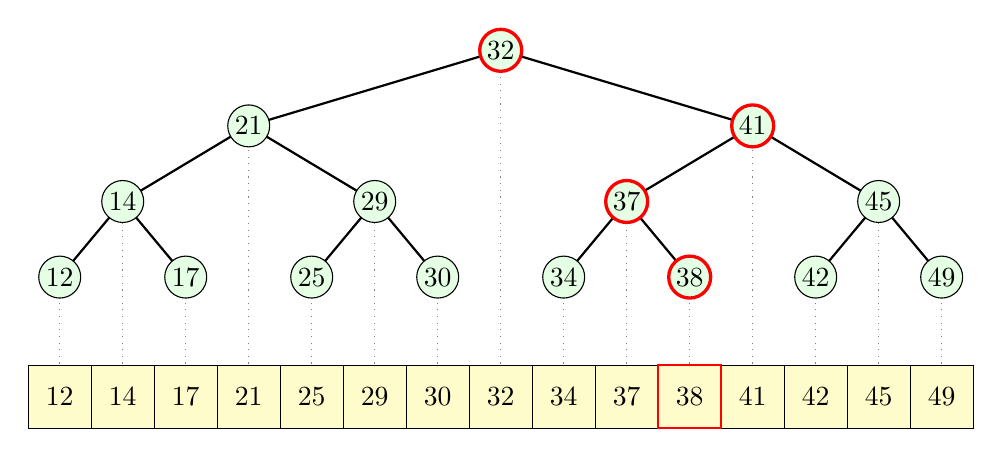
\begin{tikzpicture}[scale=0.8]
  \foreach \h[count=\i] in {1,2,1,3,1,2,1,4,1,2,1,3,1,2,1} {
    \draw[thin,gray,dotted] (\i+0.5,0.5) -- (\i+0.5,1.2+1.2*\h) coordinate (tmp-\i);
 
  }

  \foreach \i/\d  in {2/1,4/2,6/1,8/4,10/1,12/2,14/1} {
    \pgfmathtruncatemacro{\prev}{\i-\d}
    \pgfmathtruncatemacro{\next}{\i+\d}
    \draw[thick] (tmp-\prev) -- (tmp-\i) -- (tmp-\next);
  }

  \foreach \v [count=\i] in { 12,14,17,21,25,29,30,32,34,37, 38,41,42,45,49} {
    \filldraw[fill=yellow!20!white](\i,0) rectangle node[anchor=center]{\vb{\v}} (\i+1,1);

    \filldraw[fill=green!10!white] (tmp-\i) circle (2.2ex) node [anchor=center] {\vb{\v}};
  }
  
  \draw[thick,red] (11,0) rectangle (12,1);
  \foreach \i in {8,12,10,11} {
    \draw[very thick,red] (tmp-\i) circle(2.2ex);
  }

\end{tikzpicture}}


Keď chceme nájsť číslo $38$, najprv sa pozrieme do stredu, porovnám s číslon $32$, keďže
$38>32$, vydáme sa vpravo, porovnáme so $41$ atď. Našim cieľom teraz bude vyrobiť si takýto
rozhodovací strom v pamäti pomocou smerníkov. Keď sa pozrieš na obrázok, vidiš, že strom\indexItem{Alg}{binárny vyhľadávací strom}
sa skladá z krúžkov, ktoré budem volať {\em uzly} alebo {\em vrcholy}. V každom uzle 
je číslo, ktorému budem hovoriť {\em kľúč}. Najvyšší uzol v strede (na obrázku $32$) 
bude {\em koreň}, uzly naspodu budú {\em listy}. Z každého uzla okrem listu vedú 
dve čiary ({\em hrany}), ktoré vedú do koreňov menších stromov (tým hovoríme
{\em synovia} uzla). Najdlhšia vzdialenosť od koreňa do nejakého listu sa volá 
{\em hĺbka}. Základná vlastnosť,
ktorá umožňuje binárne vyhľadávanie, je to, že v celom strome aj vo všetkých podstromoch
platí: \cmd{keď si zoberiem hocijaký vrchol $v$, tak všetky kľúče v podstrome, ktorého koreň 
je ľavý syn $v$, sú menšie ako kľúč vo $v$
a všetky kľúče v podstrome, ktorého koreň je pravý syn $v$, sú zase väčšie}. 
Takýto strom budeme volať {\em binárny vyhľadávací strom}.
Spravme si takýto typ:

\begin{lstlisting}
struct Node {
  int key;
  Node *left, *right;

  Node(int _key = 0, Node *_l = nullptr, Node *_r = nullptr) {
    key = _key;
    left = _l;
    right = _r;
  }

  ~Node() {
    if (left != nullptr) delete left;
    if (right != nullptr) delete right;
  }

};
\end{lstlisting}


Vyzerá veľmi podobne ako pri spájanom zozname, len má dva pointre (na ľavého 
a pravého syna). 
Pridal som navyše deštruktor: ak sa ide z pamäti odstrániť
premenná typu \vb{Node} (či už pri volaní \prg!delete! alebo inak), najprv sa
zavolá deštruktor, ktorý sa pozrie, že existuje ľavý a/alebo pravý syn a ak áno,
rekurzívne ich zmaže (t.j. zavolá sa deštruktor ľavého syna, ktorý zavolá deštruktor
jeho synov atď), až sa zmaže celý strom. 


Ak máme utriedené pole prvkov, môžeme z neho vyrobiť strom napríklad takto:

\vbox{
  \begin{lstlisting}
Node *vyrob(vector<int> &a, int i, int j) {
  Node *res = new Node();
  if (i == j) {
    res->key = a[i];
  } else {
    int m = (i + j) / 2;
    res->key = a[m];
    if (i != m) res->left = vyrob(a, i, m - 1);
    if (m != j) res->right = vyrob(a, m + 1, j);
  }
  return res;
}
  \end{lstlisting}
}


Funkcia \vb{vyrob} má ako parametre referenciu na vektor a dva indexy \vb{i}
a \vb{j} a vyrobí strom, ktorý bude mať kľúče z úseku \prg!a[i]!\ldots\prg!a[j]!
(vrátane): zistí sa stredný prvok \vb{a[m]} a ak je ľavý alebo pravý úsek neprázdny,
rekurzívne sa zavolá \vb{vyrob} a novovytvorené podstromy sa priradia do pointrov
\vb{left} a \vb{right}. Ak mám napr. pole \vb{[10, 11, 14, 16, 20, 32, 42, 47, 50]}
a zvolám \prg!Node *root = vyrob(a, 0, a.size()-1);!, vyrobí sa v pamäti
takáto štruktúra z pointrov:

    \def\tnode(#1)[#2]#3{
      \begin{scope}[shift={(#1)}, xscale=1.3*0.7, yscale=0.7]
        \filldraw [\nodecolor, rounded corners=3pt, fill=white ] 
        (-0.5,-0.5) rectangle (0.5,0.5)
        (-0.5,0) -- (0.5,0)
        (0,0) -- (0,-0.5)
        (0,0.25) node [anchor=center]{\textcolor{magenta}{\vb{#3}}}
        (-0.25,-0.25) node[anchor=center] {\scriptsize {$\bullet$}}
        (0.25,-0.25) node[anchor=center] {{\scriptsize $\bullet$}}
        ;
        \coordinate (#2l) at (-0.25,-0.25);
        \coordinate (#2r) at (0.25,-0.25);
        \coordinate (#2) at (0,0.5);
        \coordinate (#2h) at (-0.5,0);
      \end{scope}
    }


\centerline{
  \begin{tikzpicture}[scale=0.8]
    {\small
    \def\nodecolor{cyan!50!blue}
    \foreach \h[count=\i] in {1,2,1,3,1,2,1,4,1,2,1,3,1,2,1} {
      \coordinate (tmp-\i) at (0.9*\i,0.15*\h*\h+0.8*\h) ;
    }

    \foreach \v/\c[count=\i] in {10/2, 11/4, 14/6, 16/7, 20/8, 32/10, 42/12, 47/14, 50/15} {
      \tnode(tmp-\c)[n\i]{\v}
    }

    
    \foreach \a/\b in {n2l/n1,n2r/n3,n3r/n4,n5l/n2,n5r/n7,n7l/n6,n7r/n8,n8r/n9} {
      \draw[\nodecolor,->,shorten >= 0.2ex] (\a) to[out=270,in=90] (\b);
    }
    \draw[\nodecolor,->,shorten >= 0.2ex, shorten <= 0.5ex ] ($(n5)+(0,0.5)$)
    node[anchor=south]{\vb{root}} -- (n5);
    }
  \end{tikzpicture}
}



Keď chceme zistiť, či sa nejaký kľúč v strome nachádza, stačí prechádzať stromom 
od koreňa (napr. \prg!root->find(42);!). 
Metóda \vb{find} vráti pointer na uzol s daným kľúčom,
alebo \prg!nullptr!, ak sa tam kľúč nenachádza. 

\begin{lstlisting}
struct Node {
  int key;
  Node *left, *right;
  Node(int _key = 0, Node *_l = nullptr, Node *_r = nullptr) {...}
  ~Node() {...}

  Node *find(int x) {
    if (x == key) return this;
    if (x < key && left != nullptr) return left->find(x);
    if (x > key && right != nullptr) return right->find(x);
    return nullptr;
  }
};
\end{lstlisting}


Teraz sme docielili, že v pamäti máme namiesto poľa prvky pospájané smerníkmi
a môžeme v nich vyhľadávať rovnako, ako pri binárnom vyhľadávaní v poli (teda
v logaritmickej zložitosti). Oproti binárnemu vyhľadávaniu v poli sme si ale pomohli v tom, že aj pridanie prvku má logaritmickú
zložitosť: jednoducho ideme po strome, ako keby sme vyhľadávali, a keď prídeme
na koniec, vyrobíme nový uzol. Metóoda \vb{insert} vráti \prg!true!, ak sa vrchol
v skutočnosti pridal a \prg!false!, ak už v strome bol:\\

\vbox{
\begin{lstlisting}
struct Node {
  int key;
  Node *left, *right;
  Node(int _key = 0, Node *_l = nullptr, Node *_r = nullptr) {...}
  ~Node() {...}
  Node *find(int x) {...}

  bool insert(int x) {
    if (x == key) return false;
    if (x < key && left != nullptr) return left->insert(x);
    if (x > key && right != nullptr) return right->insert(x);
    Node *nd = new Node(x);
    if (x < key) left = nd;
    else right = nd;
    return true;
  }

};
\end{lstlisting}
}

Zdá sa, že všetko funguje, a to je podozrivé. A naozaj. Keď začneš s jednoprvkovým
poľom \vb{[10]} a postupne voláš \vb{insert} pre $11, 14, 16, 20, 32, 42, 47, 50$,
v pamäti to bude vyzerať takto:


\centerline{
  \begin{tikzpicture}[scale=0.8]
    {\small
    \def\nodecolor{cyan!50!blue}

    \foreach \v[count=\i] in {10, 11, 14, 16, 20, 32, 42, 47, 50} {
      \tnode(\i,0-\i)[n\i]{\v}
    }

    
    \foreach \i in {1,...,8} {
      \pgfmathtruncatemacro{\j}{\i+1}
      \draw[\nodecolor,->,shorten >= 0.2ex] (n\i r) to[out=270,in=90] (n\j);
    }
    \draw[\nodecolor,->,shorten >= 0.2ex, shorten <= 0.5ex ] ($(n1)+(0,0.5)$)
    node[anchor=south]{\vb{root}} -- (n1);
    }
  \end{tikzpicture}
}


Takže mám obyčajný spájaný zoznam a vyhľadávanie má lineárnu zložitosť.
Problém je, samozrejme, v tom, že pridanie prvku môže spôsobiť, že strom 
prestane byť {\em vyvážený}, t.j. prestane platiť, že v každom uzle je hĺbka
ľavého a pravého podstromu skoro rovnaká. Tomu sa dá zabrániť tak, že po 
každom vložení prvku sa zavolá {\em vyvažovacia operácia}, ktorá zabezpečí, 
že strom bude ''rozumne''\footnote{%
t.j. tak, aby bolo zaručené, že operácie majú logaritmickú zložitosť}
vyvážený. Je veľa spôsobov, ako toto vyvažovanie urobiť (AVL stromy, Red-Black stromy,
\ldots). Ukážem ti jeden spôsob, zvaný AA stromy. \indexItem{Alg}{AA stromy}


Celý prístup vyzerá takto: najprv si poviem pravidlá, ktoré musí AA strom spĺňať. Potom
sa presvedčím, že každý strom, ktorý tieto pravidlá spĺňa, má logaritmickú hĺbku. Nakoniec
naprogramujem operácie (vkladanie, vyhľadávanie, mazanie) tak, aby udržovali splnené pravidlá
a navyše ich zložitosť bola úmerná hĺbke. Tak poďme na to.


V AA-strome má každý uzol okrem kľúča aj ''poschodie'' ({\em level}). Pre zjednodušenie
použijeme techniku zarážky a vyrobíme jeden špeciálny uzol {\em ''prízemie''}, ktorý bude na 
leveli 0. Pravidlá pre dobrý AA-strom sú takéto:\\



\centerline{\fcolorbox{magenta}{magenta!3!white}{\parbox{0.9\textwidth}{
\begin{enumerate}\itemsep=-1mm
\item Je to binárny vyhľadávací strom: v každom uzle platí, že všetky uzly v ľavom podstrome
  majú menšie kľúče a všetky uzly v pravom podstrome väčšie.
\item Každý uzol (okrem prízemia) má dvoch synov. 
\item \label{aarule3} Ľavý syn je na leveli o 1 menšom ako rodič.
\item Pravý syn je na rovnakom alebo o 1 menšom leveli ako rodič.
\item \label{aarule5} 
  Ak je pravý syn na rovnakom leveli ako rodič, jeho pravý syn je na menšom leveli.
\end{enumerate}
}}}

 Pravidlo~\ref{aarule5} hovorí, že nemôžu byť na rovnakom leveli tri uzly
rodič -- pravý syn -- jeho pravý syn. Zároveň, keďže prízemie má level 0, tak
podľa pravidla~\ref{aarule3}, listy musia byť na leveli 1 atď. AA-strom teda vyzerá nejak 
takto (farebné pásy sú levely):\\


\def\level(#1:#2)[#3]#4 {
  \fill[fill=#3] (\levelmin,#1) rectangle (\levelmax,#2);
}


\centerline{
  \begin{tikzpicture}[
      nodelink/.style={#1, ->, shorten >= 0.2ex},
      nodelink/.default={cyan!50!blue},
      scale=0.8]
    {\small

    \def\levelmin{-0.7}
    \def\levelmax{18.2}
    \level(-1:0.9)[green!10!white]{}
    \level(0.9:2.7)[yellow!10!white]{}
    \level(2.7:4.5)[orange!10!white]{}
    \level(4.5:6.4)[red!10!white]{}

    \def\nodecolor{cyan!50!blue}
    \foreach \x/\y/\v[count=\i] in {
      0/0.1/1,1/-0.1/2,2/0.1/4,3/-0.1/5,4/0.1/7,5/0.1/9,6/0.1/11, 7/0.1/13,8/0.1/15,
    9/0.1/17,10/0.1/19,11/-0.1/20,12/0.1/22,13/-0.1/23,14/0.1/25,
    1.5/1.1/3, 3/0.9/6, 5.5/1/10, 7.5/1.1/14, 8.5/0.9/16, 11.5/1.1/21, 12.55/0.9/24,
    4.5/2.12/8,9.5/2.12/18, 7.5/3.25/12
    } {
      \tnode(1.25*\x,1.8*\y)[n\i]{{\v}}
    }

    \coordinate (base) at (8.75,-1.7);
    \foreach \i/\d in {1/l,2/l,2/r,3/l,4/l,4/r,5/l,5/r,6/l,6/r,7/l,7/r,8/l,8/r,9/l,9/r,10/l,
    10/r,11/l,12/l,12/r,13/l,14/l,14/r,15/l,15/r} 
      \draw[gray,very thin] (n\i\d) 
      .. controls ($ (n\i\d) + (0,-1.3) $) ..
    (base);
  

    \foreach \a/\b in {16l/1,17l/3,17r/5,18l/6,18r/7, 19l/8,20l/9,20r/10,21l/11,22l/13,22r/15,
    23l/16,23r/18,24l/19,24r/21,25l/23,25r/24}
    \draw[nodelink=\nodecolor](n\a) to [out=270,in=90](n\b);

    \foreach \a/\b in {1/2, 3/4,11/12,13/14,16/17,19/20,21/22}
    \draw[nodelink=\nodecolor](n\a r) to [out=0,in=180](n\b h);

    \def\nodecolor{gray}
    \tnode(base)[tmp]{  }

    }
  \end{tikzpicture}
}



Teraz chcem vyrátať, akú najväčšiu hĺbku môže mať AA strom, v ktorom je $n$ uzlov. Spomeň si,
že hĺbka je dĺžka najdlhšej cesty z koreňa do nejakého listu. Keď začnem z koreňa a postupujem
smerom k listu, tak nikdy nejdem na vyšší level: buď idem na nižší (napr. z $18$ do
$14$) alebo ostávam na tom istom (napr. zo $14$ do $16$). Ale takisto nemôžem ísť
cez viac ako dva uzly na jednom leveli. Takže hĺbka je najviac dvojnásobok počtu levelov.
Dobre. Poďme teda vyrátať, koľko najviac levelov môže mať AA-strom, ktorý má $n$ uzlov. 
Najprv sa opýtam tak trochu opačnú otázku: 
koľko najmenej listov môže mať AA-strom, ktorý má $\ell$ levelov?
Koreň je na najvyššom leveli (teda na leveli $\ell$). 
Jeho ľavý syn je koreň AA-stromu s $\ell-1$ levelmi. Ak je
pravý syn koreňa na nižšom leveli, tak je tiež
koreňom nejakého (iného) AA-stromu s $\ell-1$ levelmi.
Ak je pravý syn koreňa na rovnakom leveli (na leveli $\ell$), tak jeho ľavý syn je koreň 
AA-stromu s $\ell-1$ levelmi. V každom prípade, v AA-strome s $\ell$ levelmi
viem nájsť dva rôzne AA-stromy
s $\ell-1$ levelmi. Preto ak si označím $L(\ell)$ najmenší počet listov, ktorý môže
mať AA-strom s $\ell$ levelmi, tak $L(\ell)\ge2L(\ell-1)$.
Dostávam teda $L(1)=1$, $L(2)\ge2$, $L(3)\ge4$, $L(4)\ge8$, \ldots, t.j. 
$L(\ell)\ge2^{\ell-1}$. Teda AA-strom s $\ell$ levelmi musí mať aspoň $2^{\ell-1}$
uzlov. Vráťme sa teraz k pôvodnej otázke: koľko najviac levelov má AA-strom s $n$ uzlami?
Keby ich mal aspoň $2+\log n$, tak by musel mať 
$L(2+\log n)\ge2^{2+\log n-1}=2n$ listov. To ale nemôže, lebo má len $n$ uzlov. Takže
AA-strom s $n$ uzlami musí mať menej ako $2+\log n$ levelov, a preto má aj logaritmickú hĺbku.


Ostáva už len posledné: naprogramovať vkladanie, vyberanie a vyhľadávanie do AA-stromu tak,
aby ich zložitosť zodpovedala hĺbke stromu. Keďže AA-strom je binárny vyhľadávací strom,
vyhľadávanie je ľahké. Najprv si spravím typ \prg!Node! podobne ako predtým. Rozdiel
bude v tom, že uzol si navyše bude pamätať svoj level. Konštruktor aj metóda
\prg!find! okrem kľúča dostanú aj pointer na prízemie (\prg!base!).
Namiesto deštruktora budem mať funckiu \prg!destroy!, lebo deštruktory nemôžu
mať parametre a ja potrebujem vedieť, čo je zarážka.


\begin{lstlisting}
struct Node {
  int level, key;
  Node *left, *right;

  Node(int k, Node *base) { level = 1; key = k; left = right = base; }

  void destroy(Node *base) {
    if (this == base) return;
    left->destroy(base);
    right->destroy(base);
    delete this;
  }

  bool find(int k, Node *base) {
    if (this == base) return false;
    if (key == k) return true;
    if (k < key)
      return left->find(k, base);
    else
      return right->find(k, base);
  }
};
\end{lstlisting}

Urobím si aj nový typ \prg!Tree! pre celý strom, v ktorom budem mať zapamätaný koreň
a prízemie:


\begin{lstlisting}
struct Tree {
  Node *root, *base;

  Tree() {
    base = new Node(0,nullptr); // vyrobím si prízemie
    base->level = 0;
    base->left = base->right = base;
    root = base; 
  }

  ~Tree() { root->destroy(base); delete base; }

  bool find(int key) { return root->find(key, base); }
};
\end{lstlisting}


Pridávanie ale začne byť trochu komplikovanejšie. Zoberme si jednoduchú funkciu \vb{insert}
z predchádzajúceho prípadu. Začnem s prázdnym stromom a pridám doňho čísla $9$ a $20$. Bude to vyzerať nejak takto (modré číslo znamená level, čiarkovaná čiara je prízemie):

%\tikzset{external/force remake}
\def\aaangle{17}
\def\aanormalcolor{yellow!7!white}
\def\aanode(#1)#2#3{%
  \filldraw[thick, fill=\aanormalcolor] (#1) node {#2} circle (2.2ex) 
        ++ (1ex,1ex) node [anchor=south west] {\textcolor{blue}{{\small\roboto #3}}} ;
  }
\def\aasub(#1)#2#3{%
  \coordinate(tmp1) at ($(#1)+(270-16:1.3)$);
  \coordinate(tmp2) at ($(#1)+(270+16:1.3)$);
  \filldraw[thick, fill=green!7!white] 
      (#1) -- (tmp1) -- (tmp2) -- (#1);
  \def\tmpr{1.8ex}    
  \filldraw[thick, fill=green!7!white] 
      ($(#1)+(-\tmpr,-\tmpr)$) rectangle 
      node[align=center] {\vb{#2}} 
      ($(#1)+(\tmpr,\tmpr)$) 
      ($(#1)+ (\tmpr,\tmpr)$) node[anchor=south west]  {\textcolor{blue}{{\small\roboto #3}}} ;
  }
\def\ground(#1)#2{
  \coordinate (tmp1) at ($(#1)+(270#2\aaangle:5)$);
  \coordinate (tmp2) at (intersection of #1--tmp1 and {-10,0}--{10,0});
  \draw(#1)--(tmp2);
}
\centerline{
  \begin{tikzpicture}
    \foreach\x/\y[count=\i]in{0/1,1/0.87} 
      \coordinate (n\i) at (1.5*\x,1.5*\y);
  
    \draw[dashed](-1,0)--(2.5,0);
    \ground(n1)-
    \ground(n2)-
    \ground(n2)+
    \draw(n1)--(n2);
    \draw (n1) -- +(0,0.7);
    \aanode(n1){9}{1}
    \aanode(n2){20}{1}
  \end{tikzpicture}
}


Keď chcem pridať číslo $15$, vznikne problém:

\centerline{
  \begin{tikzpicture}
    \foreach\x/\y[count=\i]in{0/1.4,1.6/1.2,1/0.5} 
      \coordinate (n\i) at (\x,1.5*\y);

    \draw[dashed](-1.2,0)--(2.7,0);
    \ground(n1)-
    \ground(n2)+
    \ground(n3)-
    \ground(n3)+
    \draw(n1)--(n2) --(n3);
    \draw(n1) -- +(0,0.7);
    \aanode(n1){9}{1}
    \aanode(n2){20}{1}
    \aanode(n3){15}{1}
  \end{tikzpicture}
}


Uzol $15$ musí byť na leveli 1, lebo je to list, ale zároveň je ľavým synom uzla $20$, preto
$20$ musí mať level $2$. Lenže pravý syn $20$ky je prízemie (s levelom 0), preto
$20$ musí mať level $1$. Takže je zrejmé, že nestačí len aktualizovať levely, ale bude treba 
prerobiť aj celý strom. V tomto príklade môžem na uzol $20$ použiť operáciu {\em skew} 
({\em rotácia}), ktorá vyzerá takto:


\centerline{\begin{tikzpicture}
\foreach\x/\y[count=\i]in{0/0, 1.4/0, 0.7/1.35, 2.2/1.8, 3/0}
      \coordinate (n\i) at (\x,\y);
      
\draw (n1) -- (n3) -- (n2) (n3)--(n4)--(n5) (n4) -- ++(0,0.7);   
\aanode(n3){$x$}{k}
\aanode(n4){$y$}{k}
\aasub(n1){$A$}{k-1}
\aasub(n2){$B$}{k-1}
\aasub(n5){$C$}{k-1}

\node[draw, single arrow, minimum height=22mm, minimum width=8mm,
  single arrow head extend=2mm, anchor=center] at (5.5,0.7) {};

\begin{scope}[shift={(8,0)}]
  \foreach\x/\y[count=\i]in{0/0, 1.6/0, 0.7/1.8, 2.2/1.35, 3/0}
      \coordinate (n\i) at (\x,\y);
      
  \draw (n1) -- (n3) --(n4) (n2)--(n4)--(n5) (n3) -- ++(0,0.7);   
  \aanode(n3){$x$}{k}
  \aanode(n4){$y$}{k}
  \aasub(n1){$A$}{k-1}
  \aasub(n2){$B$}{k-1}
  \aasub(n5){$C$}{k-1}
\end{scope}

\end{tikzpicture}}



Povedané slovami: ak mám podstrom s koreňom $y$ na leveli $k$, 
ktorý má ľavého syna $x$ na leveli $k$ (čím
sa porušilo pravidlo~\ref{aarule3}) a $x$ má obidvoch synov na leveli $k-1$, môžem 
za koreň podstromu zvoliť $x$ a pravého syna $x$ prevesiť pod $y$. Po operácii posun
strom ostane dobrý vyhľadávací strom, lebo všetky kľúče v podstrome $B$ sú menšie ako $y$.
Operáciu \prg!skew! si naprogramujem ako metódu \prg!Node!. Zavolám ju v koreni
podstromu (napr. \prg!root=root->skew()!) a bude vracať
pointer na nový koreň stromu:

\begin{lstlisting}
Node *skew() {
  if (left->level != level) return this;
  Node *res = left, *tmp = left->right;
  left->right = this;
  left = tmp;
  return res;
}
\end{lstlisting}


Ak aplikujem \vb{skew} na uzol $20$ z príkladu, dostanem 

\centerline{
  \begin{tikzpicture}
    \foreach\x/\y[count=\i]in{0/1.4,1.6/1.2,1/0.5} 
      \coordinate (n\i) at (\x,1.5*\y);

    \draw[dashed](-1.2,0)--(2.7,0);
    \ground(n1)-
    \ground(n2)+
    \ground(n3)-
    \ground(n3)+
    \draw(n1)--(n2) --(n3);
    \draw(n1) -- +(0,0.7);
    \aanode(n1){9}{1}
    \aanode(n2){20}{1}
    \aanode(n3){15}{1}

    \node[draw, single arrow, minimum height=20mm, minimum width=8mm,
  single arrow head extend=2mm, anchor=center] at (4.5,1) {};


    \begin{scope}[shift={(8,0)}]
    \foreach\x/\y[count=\i]in{0/1.3, 1.7/0.5, 1.2/1} 
      \coordinate (n\i) at (\x,1.5*\y);

    \draw[dashed](-1.2,0)--(2.7,0);
    \ground(n1)-
    \ground(n2)+
    \ground(n2)-
    \ground(n3)-
    \draw(n1)--(n3) --(n2);
    \draw(n1) -- +(0,0.7);
    \aanode(n1){9}{1}
    \aanode(n2){20}{1}
    \aanode(n3){15}{1}
    \end{scope}
  \end{tikzpicture}
}


Teraz som vyriešil problém v pravom podstrome uzla $9$, ale problém je v samotnej $9$ke:
uzly $15$ aj $20$ sú na leveli 1, a tým porušujú pravidlo~\ref{aarule5}. To ošetrím druhou
operáciou, ktorú nazvem {\em split} ({\em rozdelenie}) a vyzerá takto:


\centerline{\begin{tikzpicture}
\foreach\x/\y[count=\i]in{0.7/1.8,2.1/1.6,3.5/1.4, 0/0,1.4/0,2.8/0,4.2/0}
      \coordinate (n\i) at (\x,\y);
      
  \draw (n4) -- (n1) -- (n2) -- (n3)--(n7) (n5)--(n2) (n6)--(n3) (n1) -- ++(0,0.7);   
\aanode(n1){$x$}{k}
\aanode(n2){$y$}{k}
\aanode(n3){$z$}{k}
\aasub(n4){$A$}{k-1}
\aasub(n5){$B$}{k-1}
\aasub(n6){$C$}{k-1}
\aasub(n7){$D$}{k-1}

\node[draw, single arrow, minimum height=20mm, minimum width=8mm,
  single arrow head extend=2mm, anchor=center] at (6.5,0.7) {};

\begin{scope}[shift={(9,0)}]
\foreach\x/\y[count=\i]in{0.7/1.4,2.1/1.9,3.5/1.4, 0/0,1.4/0,2.8/0,4.2/0}
      \coordinate (n\i) at (\x,\y);
      
  \draw (n4) -- (n1) -- (n2) -- (n3)--(n7) (n5)--(n1) (n6)--(n3) (n2) -- ++(0,0.7);   
\aanode(n1){$x$}{k}
\aanode(n2){$y$}{k+1}
\aanode(n3){$z$}{k}
\aasub(n4){$A$}{k-1}
\aasub(n5){$B$}{k-1}
\aasub(n6){$C$}{k-1}
\aasub(n7){$D$}{k-1}
\end{scope}

\end{tikzpicture}}


Slovami, ak mám postupne dvoch pravých synov na rovnakom leveli ako rodič, môžem stredného
posunúť na vyšší level. Opäť to naprogramujem rovnako, ako predtým, t.j. ako metódu,
ktorá vracia pointer na nový koreň:


\begin{lstlisting}
 Node *split() {
    if (right->right->level != level) return this;
    right->level++;
    Node *res = right;
    right = right->left;
    res->left = this;
    return res;
  }
\end{lstlisting}

Keď aplikujem \vb{split} na vrchol $15$, výsledný strom bude

\centerline{
  \begin{tikzpicture}
    \foreach\x/\y[count=\i]in{0/1.3, 1.7/0.5, 1.2/1} 
      \coordinate (n\i) at (\x,1.5*\y);

    \draw[dashed](-1.2,0)--(2.7,0);
    \ground(n1)-
    \ground(n2)+
    \ground(n2)-
    \ground(n3)-
    \draw(n1)--(n3) --(n2);
    \draw(n1) -- +(0,0.7);
    \aanode(n1){9}{1}
    \aanode(n2){20}{1}
    \aanode(n3){15}{1}

\node[draw, single arrow, minimum height=20mm, minimum width=8mm,
  single arrow head extend=2mm, anchor=center] at (4.5,1) {};

\begin{scope}[shift={(8,0)}]

    \foreach\x/\y[count=\i]in{0/0.5, 1.6/0.5, 0.8/1.4} 
      \coordinate (n\i) at (\x,1.5*\y);

    \draw[dashed](-1.2,0)--(2.7,0);
    \ground(n1)-
    \ground(n2)+
    \ground(n2)-
    \ground(n1)+
    \draw(n1)--(n3) --(n2);
    \draw(n3) -- +(0,0.7);
    \aanode(n1){9}{1}
    \aanode(n2){20}{1}
    \aanode(n3){15}{2}
\end{scope}
  \end{tikzpicture}
}
%\tikzset{external/force remake=false}


Pridaním listu a následným volaním \vb{skew} a \vb{split} sa mi mohlo stať, že
sa porušia pravidlá vyššie v strome. V mojom príklade je teraz koreň namiesto 
uzla $9$ s levelom $1$, uzol $15$ s levelom $2$. Keby to nebol celý strom, ale 
nad ním by bol napr. uzol $30$ s levelom $2$, porušilo by sa mi v ňom pravidlo~\ref{aarule3}.
Možnosti, ako sa to môže stať, sú ale rovnaké, ako pri pridávaní listu\footnote{%
  všimni si, že jediné miesto, kde level môže stúpnuť, je pri operácii \vb{split},
  ale potom sú obaja synovia na menšom leveli}. Preto celé pridávanie môžem napísať
  jednoducho takto:

\begin{lstlisting}
struct Node {
  int level, key;
  Node *left, *right;

  Node(int k, Node *base) { ... }
  void destroy(Node *base) { ... }
  bool find(int k, Node *base) { ... }
  
  Node *skew() { ... }
  Node *split() { ... }

  Node *insert(int k, Node *base) {
    if (this == base) return new Node(k, base);
    if (k == key) return this;
    if (k < key)
      left = left->insert(k, base);
    else
      right = right->insert(k, base);
    return skew()->split();
  }
};

struct Tree {
  Node *root;
  Node *base;

  Tree() { ... }
  ~Tree() { ... }

  void insert(int key) { root = root->insert(key, base); }
  bool find(int key) { return root->find(key, base); }
};

\end{lstlisting}


Uzly, ktoré sú v strome, sa dajú odstrániť podobným spôsobom. Ak mám odstrániť list,
nájdem ho ako pri vyhľadávaní, zmažem ho, a po zmazaní dovyvažujem strom. Problém je,
čo urobiť, ak mám vymazať uzol, ktorý nie je list. Pomôže drobná finta: ak mám
vymazať uzol $x$, ktorý má ľavého syna, nájdem si uzol $y$ s najväčším kľúčom v podstrome
ľavého syna (t.j. najpravejší list). Viem, že $y$ je väčší, ako všetky kľúče v ľavom podstrome
$x$ a zároveň menší, ako všetky kľúče v pravom podstrome. Môžem teda vymeniť hodnoty
$x$ a $y$, a už mi stačí vymazať list. Ak $x$ nemal ľavého syna, ale iba pravého, 
urobím to symetricky (hľadám najľavejší list). V súbore 
\link{\rootpath/aatree.h}{aatree.h}
je strom aj s dopísanou operáciou \vb{erase}: pri postupe smerom nadol
si v premennej \vb{deleted} uchovávam posledný uzol, ktorého kľúč je $\ge k$. Keď
prídem do príslušného listu (najľavejšieho alebo najpravejšieho), tak vymením
hodnoty a dovyvažujem strom (skús si premyslieť, ako to funguje).


Vráťme sa teraz k úlohe o žiarovkách s výrobnými číslami.
S použitím AA stromu je to ľahké.

\begin{uloha}
  \label{uloha:ziarovky-vela}
  Na vstupe je  postupnosť príkazov. Každý príkaz je tvaru
  \vb{! x} alebo \vb{? x} a posledný príkaz je \vb{\#}. 
  Predpokladajme, že máme žiarovky, 
  ktoré su na začiatku vypnuté. Príkaz \vb{! x} znamená, že sme prepli žiarovku
  s výrobným číslom $x$ (ak bola vypnutá, bude zapnutá a naopak). Pre každý príkaz \vb{? x}
  treba vypísať, \vb{svieti} alebo \vb{nesvieti} podľa toho, v akom stave je práve žiarovka
  číslo $x$.
\end{uloha}

Skús si napísať rekurzívnu funkciu na nasledujúcu úlohu:

\begin{uloha}
  Napíš funkciu, ktorá vypíše všetky kľúče z AA stromu v utriedenom poradí.
\end{uloha}



V STL sú podobné stromy naprogramované v type, ktorý sa volá {\em monžina} ({\em set}).\indexItem{Prg}{\vb{set}} 
Na použitie treba pridať \prg!#include <set>!.
Je to šablóna, ktorá má ako parameter typ kľúča, takže napr. \prg!set<int> s;! je
strom, ktorý má 
kľúče typu \prg!int!. Namiesto \prg!int! to môže byť hocijaký iný typ, ktorý má definované
porovnanie. Pri vlastných typoch treba \prg!operator<! definovať ako \prg!const!,
napr. takto:

\begin{lstlisting}
struct Osoba {
  string meno, priezvisko;

  bool operator<(const Osoba& x) const {
    if (priezvisko == x.priezvisko) return meno < x.meno;
    return priezvisko < x.priezvisko;
  }
};
\end{lstlisting}

\prg!const! pri parametri \vb{x} 
znamená, že \vb{x} je referencia na premennú typu \vb{Osoba},
ale funkcia \prg!operator<! sľubuje, že \vb{x} nebude meniť. Podobne \prg!const! za menom
funkcie sľubuje, že sa nebude meniť \prg!*this!, t.j. ak zavolám \prg!x.operator<(y)!,
tak sa nezmení ani \vb{x} ani \vb{y}. 
Pri takejto definícii môžem použiť \prg!set<Osoba>! a budem mať v strome osoby utriedené podľa
priezviska a pri rovnakom priezvisku podľa mena.


Iná možnosť je použiť šablónu \vb{set}
s dvoma parametrami, kde druhý parameter je typ porovnávacej
funkcie, a porovnávacia funkcia je potom parametrom konštruktora. 
Keby typ \vb{Osoba} nemal definované porovnanie, alebo keby som chcel
mať strom usporiadaný najprv podľa mena a potom podľa priezviska, môžem napísať
(potrebujem pridať \prg!#include <functional>!):

\begin{lstlisting}
set<Osoba, function<bool(const Osoba &, const Osoba &)>> s(
    [](const Osoba &x, const Osoba &y) {
      if (x.meno == y.meno) return x.priezvisko < y.priezvisko;
      return x.meno < y.meno;
    });
\end{lstlisting}

Tým hovorím, že chcem vyrobiť vyhľadávací strom s uzlami s hodnotou \vb{Osoba} a na 
porovnávanie budem používať funkciu (lambdu), ktorá zoberie referencie na dve premenné
typu \vb{Osoba} a vráti \prg!bool!.


Podobne ako v našom type \vb{Tree}, typ \prg!set! má
operácie \prg!s.insert(x)! a \prg!s.erase(x)!. Keďže je to kontajner, má 
definované aj iterátory\footnote{Na rozdiel od vektora, iterátor pre \prg!set! sa
dá posunúť len na susedný prvok, t.j. môžem mať \prg!it++! alebo \prg!it--!, ale 
nie \prg!it+10!}, takže napr.

\begin{lstlisting}
for (auto it = s.begin(); it != s.end(); it++) cout << *it << " ";
\end{lstlisting}

vypíše všetky prvky. Navyše je zaručené, že pri prechode iterátorom
budú prvky usporiadané od najmenšieho po najväčší. Vyhľadávanie prvku robí
metóda \vb{find(x)}, ktorá vráti iterátor na prvok s kľúčom \vb{x}, 
alebo \vb{end()}, ak tam 
prvok s daným kľúčom nie je.
Takže zistiť, či je kľúč \vb{x} v množine, sa dá pomocou \prg~if (s.find(x) != s.end())~
Metóda \vb{erase} má dve verzie: buď vymaže prvok s daným kľúčom alebo prvok s
daným iterátorom. Napr. \prg!s.erase(s.begin())! vymaže najmenší prvok.
Hodí sa ešte funkcia \prg!upper_bound(x)! (resp. \prg!lower_bound(x)!), ktorá vráti
iterátor na najmenší prvok väčší (resp. väčší alebo rovný) ako \prg|x|.


Ako presne je \prg!set! naprogramovaný je na konkrétnom kompilátore, ale musí zaručiť,
aby zložitosť všetkých operácií (vyhľadávanie, vkladanie, mazanie) bola logaritmická.
Existujúce kompilátory väčšinou používajú
tzv. {\em Red-Black} stromy, ktoré majú trochu iný spôsob vyvažovania, ale v podstate
sú veľmi podobné AA stromom. 
V nasledovnom grafe je porovnanie časov. Pre rôzne hodnoty $n$ som
povkladal do stromu $n$ rôznych čísel (v náhodnom poradí) a potom som ich (v náhodnom poradí)
zo stromu vymazal. Meral som si priemerný čas, ktorý trvala jedna operácia. Vidno, že
\prg!set! je trochu rýchlejší\footnote{a aj konzistentnejší, modrá krivka je viac roztrasená}, 
ako náš \vb{Tree}, ale zase nie až tak o veľa. V obidvoch
prípadoch rastie čas, ktorý treba na vloženie (vymazanie) iba veľmi pomaly 
v závislosti od veľkosti stromu.



\begin{tikzpicture}
\begin{axis}[
  width=\textwidth, 
  height=10cm,
  xlabel=$n$,
  ylabel=čas ($\mu$s),
  legend cell align={left},
  legend pos = north west,
  %  scaled x ticks=false,
  %scaled y ticks=false,
    /pgf/number format/.cd,
        1000 sep={}
]
  \addplot+[blue!80!white, 
  line join=round, mark size=0.5pt] table [y=aa, x=n]{data/tree_test.dat};
  \addlegendentry{\vb{aatree.h}}
  \addplot+[orange!80!white, 
  line join=round, mark size=0.5pt] table [y=set, x=n]{data/tree_test.dat};
  \addlegendentry{\vb{set<int>}}
\end{axis}
\end{tikzpicture}





V STL je aj niekoľko podobných dátových štruktúr. \prg!multiset! sa od \prg!set!
líši tým,
že dovoľuje mať viacero prvkov s rovnakým kľúčom\footnote{%
  Tu si treba dať pozor: \prg!s.erase(x)! vymaže všetky prvky s kľúčom \prg!x!.
  Na vymazanie jedného treba použiť \prg!s.erase(s.find(x))!, t.j. nájsť iterátor 
  na nejaký konkrétny uzol s kľúčom \vb{x} a potom vymazať ten.}. 


  Podobný ako \prg!set! je aj typ \prg!map!, v ktorom každý uzol 
  má okrem kľúča aj hodnotu. Je to šablóna s dvoma parametrami, 
  napr. \prg!map<string,int> m;! používa ako kľúč
  \prg!string! \footnote{\prg!string! má definovaný operátor porovnania, ktorý dva reťazce
  porovná podľa abecedy ako slová v slovníku} a každý uzol má hodnotu typu \prg!int!.
  K uloženým hodnotám sa dá príjemne pristupovať pomocou operátora \prg![]!, podobne
  ako pri vektore, takže napr. \prg!m["zaba"]=5;! vloží do stromu uzol s kľúčom
  \prg!"zaba"! a hodnotou 5 (ak tam už uzol s takým kľúčom bol, zmení jeho hodnotu).
  Podobne \prg!x=m["zaba"];! uloží do premennej \prg!x! hodnotu, ktorá je v uzle
  s kľúčom \prg!"zaba"! (ak taký uzol nie je, tak sa vytvorí, a jeho hodnota bude 0;
  v tom prípade sa teda do \prg!x! uloží 0). 
  Metódy \prg!find! a \prg!erase! fungujú rovnako ako
  pri type \prg!set!: \prg!find! vráti iterátor na uzol s daným kľúčom a
  \prg!erase! vymaže buď uzol s daným kľúčom, alebo iterátor. 

 
 Iterátory v type \prg!map! sú trochu zložitejšie. Kým iterátor pre \prg!set! sa dá \indexItem{Prg}{iterátory pre \vb{set} a \vb{map}}
 chápať ako pointer na kľúč (napr. ak mám \prg!auto it=s.begin();!, tak \prg!*s! je 
 kľúč), iterátor na \prg!map! potrebuje ukazovať na dve veci: kľúč a hodnotu. Dať dve veci
 do jednej premennej je treba často a v STL je na to špeciálny typ \prg!pair!, \indexItem{Prg}{typ \vb{pair}}
 ktorý vyzerá takto:

\begin{lstlisting}
template<class T1, class T2>
struct pair {
  T1 first;
  T2 second;
};
\end{lstlisting}

Sú v ňom definované rôzne pomocné funkcie (napr. \prg!operator==! a pod.). Taktiež
aj funkcia (šablóna) \prg!make_pair!, kotrá ušetrí písanie \prg!<T1,T2>!. Kompilátor si totiž vie odvodiť typy, takže ak napíšeš
napr. \prg!make_pair(3,4.7)!, tak vráti \prg!pair<int,double>!.

\vskip 2ex
\vbox{
\begin{lstlisting}
template<class T1, class T2>
pair<T1, T2> make_pair(T1 x, T2 y) { 
  return pair<T1, T2>(x, y); 
}
\end{lstlisting}
}

Iterátor na \prg!map! sa správa ako pointer na \prg!pair!, kde prvá zložka je
kľúč a druhá hodnota. Napr. keby som chcel mať vyhľadávací strom, v ktorom
podľa zvuku viem nájsť živočícha, použil by som \prg!map<string,string>! napr.
takto:

\vskip 2ex
\begin{lstlisting}
#include <iostream>
#include <map>
#include <string>
using namespace std;

int main() {
  map<string, string> m;
  m["vauu"] = "vlk";
  m["mnau"] = "macka";
  m["kvak"] = "zaba";
  m["singularna kohomologia"] = "matematik";

  for (auto it = m.begin(); it != m.end(); it++)
    cout << it->second << " hovori '" << it->first << "'" << endl;
}
\end{lstlisting}

Všimni si, že program bude vypisovať živočíchy utriedené abecedne podľa zvuku, ktorý vydávajú.
No a posledná vec, iterátory na \prg!set! aj \prg!map! sú, na rozdiel od vektora \prg!const!.
Preto ak mám napr. \prg!vector<int> a;!, tak môžem napísať

\begin{lstlisting}
auto it = a.begin();
it++;
*it=10;
\end{lstlisting}

a bude to to isté, ako \prg!a[1]=10!, ak by som mal \prg!set<int> a;!, tak 
\prg!*it=10;! napísať 
nemôžem\footnote{To, samozrejme, dáva zmysel: nemôžem len tak zmeniť hodnotu v 
uzle vyhľadávacieho stromu; tým sa mi veci môžu pokaziť.}.


Predtým, ako sa pustíme do úloh, ešte jedna poznámka o zložitosti. Ukázali sme si, že \prg!set! a 
\prg!map! sú naprogramované tak, že zložitosť všetkých operácií je logaritmická. To je pravda,
ale ak to povieme presnejšie, tak logaritmický je počet volaní porovnania. Ak by si mal
napr. \prg!set<string>!, tak pri vyhľadávaní
sa v každom kroku musí porovnať hľadaný reťazec s kľúčom príslušného uzla. A to môže trvať
dosť dlho, ak máš dlhé reťazce. Takže počet porovnaní síce je logaritmický, ale jedno porovnanie
môže byť veľmi drahé. Na to si treba dávať pozor, ak používaš ako kľúč zložitejšie typy.

\begin{uloha}
  Na vstupe je číslo $n$ a potom $n$ riadkov, z ktorých každý opisuje výsledok hry.
  Riadok v tvare \vb{Jano Fero 10} znamená, že hráč \vb{Jano} vyhral od hráča \vb{Fero}
  \vb{10} tokenov (t.j. \vb{Jano} má o $10$ viac a \vb{Fero} o $10$ menej).
  Napíš program, ktorý vypíše všetkých hráčov v abecednom poradí a pre každého jeho
  záverečný zisk (t.j. kladné číslo, ak má viac tokenov ako na začiatku a záporné
  ak má menej). Napr.


\begin{column}{0.45}
\begin{outputBox}
5
Jano Fero 10
Fero Mara 42
Mara Jano 14
Dream Technoblade 20
Technoblade Fero 84
\end{outputBox}
\end{column}\hfill\begin{column}{0.45}
\begin{outputBox}
Dream: 20
Fero: -52
Jano: -4
Mara: -28
Technoblade: 64
\end{outputBox}
\end{column}
\end{uloha}


Poďme teraz spolu vyriešiť takúto úlohu:

\begin{uloha}
Máme za úlohu vykonať $n$ činností očíslovaných $0,1,\ldots,n-1$. Zároveň máme daných
  $m$ podmienok tvaru $i\overset{t}{\mapsto} j$, ktoré hovoria, že činnosť $j$
  sa dá urobiť najskôr $t$ dní po tom, ako sa urobí činnosť $i$. V jeden deň 
  sa dá urobiť hocikoľko veľa činností, ak to podmienky dovoľujú.
  Napíš program, ktorý vypíše poradie,
  v akom sa dajú činnosti vykonať, alebo napíše, že sa to nedá. Napr.


\def\nd(#1)#2{\filldraw[thick, fill=yellow!10!white] (#1) node {\vb{#2}} circle (2ex);}
\def\lnks(#1,#2)#3{\draw [->, shorten >= 2.4ex] (n#1) --  node[anchor=south]{\vb{\small #3}} (n#2);}
\def\lnk(#1,#2)#3#4{\draw [->, shorten >= 2.4ex] (n#1) to[out=#3,in=180-#3] node[anchor=south]{\vb{\small #4}} (n#2);}
\def\lnkf(#1,#2)[#3,#4]#5{\draw [->, shorten >= 2.4ex] (n#1) to[out=#3,in=#4] node[anchor=south]{\vb{\small #5}} (n#2);}

\begin{minipage}[t]{0.2\textwidth}\vspace{0pt}
\begin{Verbatim}
6 9
3 0 2
1 2 1
4 0 6
3 1 1
4 2 4
2 0 1
3 4 2
1 5 5
5 0 2
\end{Verbatim}
\end{minipage}
  \begin{minipage}[t]{0.5\textwidth}\vspace{0pt}
  \begin{tikzpicture}    
    \foreach \v [count=\i] in {3,1,4,2a,0}
    \coordinate (n\v) at (1.3*\i,0);
    \coordinate (n2) at ($(n2a)+(0,6ex)$);
    \coordinate (n5) at ($(n2a)+(0,-6ex)$);

    \lnks(3,1)1
    \lnk(3,4){50}2
    \lnks(4,0)6
    \lnks(4,2)4
    \lnks(2,0)1
    \lnks(5,0)2
    \lnkf(1,2)[70,180]1
    \lnkf(1,5)[290,180]5

    \coordinate (tmp) at ($(n4)+(0,-12ex)$);
    \draw(n3) to [out=270,in=180] (tmp);
    \draw [->, shorten >= 2.4ex] (tmp) to [out=0,in=270] (n0);
    \node[anchor=south] at (tmp) {\vb{\small 2}} ;

    \foreach \v in {5,4,3,1,2,0} {
    \nd(n\v){\v}
    }
  \end{tikzpicture}
  \end{minipage}
  \begin{minipage}[t]{0.3\textwidth}\vspace{0pt}
\begin{Verbatim}
1. den: 3
2. den: 1
3. den: 4
7. den: 5 2
9. den: 0
\end{Verbatim}
\end{minipage}

\vskip 2ex
alebo

\begin{minipage}[t]{0.2\textwidth}\vspace{0pt}
\begin{Verbatim}
4 5
0 1 1
1 2 1
1 3 1
3 2 1
2 0 1
\end{Verbatim}
\end{minipage}\begin{minipage}[t]{0.5\textwidth}\vspace{0pt}
  \begin{tikzpicture}    
    \foreach \v/\x/\y in {0/0/0,1/1.5/0,3/3/0,2/1.5/-1.2}
    \coordinate (n\v) at (\x,\y);

    \foreach \u/\v in {0/1,1/3,1/2,2/0,3/2}{
      \lnks(\u,\v)1
    }

    \foreach \v in {3,1,2,0} {
    \nd(n\v){\v}
    }
  \end{tikzpicture}
\end{minipage}\begin{minipage}[t]{0.3\textwidth}\vspace{0pt}
\begin{Verbatim}
neda sa
\end{Verbatim}
\end{minipage}

\end{uloha}

Ukážeme si jednoduché riešenie s využitím STL. Najprv si prečítam podmienky zo vstupu. Podmienka
tvaru \hbox{\vb{i j t}} reprezentuje šípku $i\overset{t}{\mapsto} j$. O každej šípke si budem
pamätať kam ide a ako dlho treba čakať. Na to si vyrobím typ \vb{Sipka}:

\vskip 1ex
\vbox{
\begin{lstlisting}
struct Sipka {
  int j, t;
};
\end{lstlisting}
}

Všetky podmienky budem mať uložené v premennej \prg!verctor<vector<Sipka>> G!. To znamená, že
\vb{G} je vektor, ktorého prvky sú zase vektory, v ktorých sú uložené šípky. \vb{G[i]}
bude vektor, v ktorom budem  mať zapamätané šípky, ktoré odchádzajú z $i$\footnote{preto som  si
v type \vb{Sipka} zapamätal iba cieľovú činnosť. Odkiaľ šípka vychádza bude dané tým,
kde je uložená.}. Na začiatku si inicializujem \vb{G} na veľkosť $n$, t.j. bdue obsahovať
$n$ prázdnych vektorov. Potom vždy prečítam jednu podmienku $i\overset{t}{\mapsto} j$
a pridám \vb{Sipka\{j,t\}} na koniec vektora \vb{G[i]} takto:

\vskip 1ex
\vbox{
\begin{lstlisting}
cin >> n >> m;
vector<vector<Sipka>> G(n);
while (m-- > 0) {
  int i, j, t;
  cin >> i >> j >> t;
  G[i].push_back(Sipka{j, t});
}
\end{lstlisting}
}

Keď mám prečítaný vstup, idem úlohu riešiť. Priamočiary prístup by bol prechádzať postupne
dni,  vždy skontrolovať, ktoré činnosti môžem urobiť, a tie urobiť\footnote{Je 
totiž jasné, že ak nejakú činnosť 
môžem urobiť, neoplatí sa ju odkladať. Keby som mal napríklad ale obmedzený počet činností, ktoré
za deň môžem urobiť, všetko by bolo úplne inak.}. Na začiatku môžem urobiť všetky činnosti,
do ktorých nevchádza žiadna šípka. Keď ich urobím, odstránim z nich odchádzajúce šípky, a tým sa mi  môžu objaviť nové činnosti, do ktorých 
žiadna šípka nevchádza. Tie ale môžem urobiť až potom, ako vyčkám patričný čas. Preto si
o každej činnosti budem pamätať dve veci: {\em stupeň}, t.j. koľko šípok do nej ešte vchádza,
 a čas, dokedy treba čakať, aby sa splnili už vybavené šípky. 
Budem mať typ

\vskip 1ex
\vbox{
\begin{lstlisting}
struct Info {
  int deg, t;
};
\end{lstlisting}
}

a \vb{vector<Info> a}, ktorý si pri čítaní vstupu nastavím takto:

\vskip 1ex
\vbox{
\begin{lstlisting}
cin >> n >> m;

vector<Info> a(n);
for (int i = 0; i < n; i++) {
  a[i].t = 0;
  a[i].deg = 0;
}

vector<vector<Sipka>> G(n);
while (m-- > 0) {
  int i, j, t;
  cin >> i >> j >> t;
  G[i].push_back(Sipka{j, t});
  a[j].deg++;
}
\end{lstlisting}
}

Spracovať udalosť \vb{i} potom znamená pre každú udalosť \vb{j}, do ktorej vedie z \vb{i} šípka, znížiť stupeň a 
upraviť čas, kedy ju môžem najskôr urobiť:

\vskip 1ex
\vbox{
\begin{lstlisting}
for (Sipka s : G[i]) {
  a[s.j].deg--;
  a[s.j].t = max(a[s.j].t, a[i].t + s.t);
}
\end{lstlisting}
}

Tu som použil nový zápis \prg!for (Sipka s : G[i]) prikaz!, ktorý je skratkou za\indexItem{Prg}{\vb{for} cyklus cez kontajner}

\vskip 1ex
\vbox{
\begin{lstlisting}
 for (auto it = G[i].begin(); it != G[i].end(); it++) {
   Sipka s = *it;
   <prikaz>
 }
\end{lstlisting}
}

Všeobecne môžem písať \prg!for( auto w : x)!, kde
 \vb{x} môže byť hocičo, čo má príslušné iterátory (\prg!vector!, \prg!set!,
\prg!map!, vlastný typ, \ldots). Namiesto vypísania typu \vb{w} môžem použiť  \prg!auto!\footnote{%
  Poznámka pre fajnšmekrov: Keby som mal napr. \prg!vector<vector<int>> G;!
  a napíšem \prg!for (auto w : G) w[0]=7;!, tak \prg!w! bude typu \prg!vector<int>!
  a pri vykonávaní neviditeľného \prg!vector<int> w = *it! vovnútri cyklu
  sa vo \vb{w} 
  vytvorí lokálna kópia vektora \prg!*it!.
  Výsledkom bude, že dáta sa budú veľakrát kopírovať a hodnoty v \vb{G} sa nezmenia.
  Ak napíšem \prg!for (auto &w : G) x[0]=7;!, tak \vb{w} bude typu \prg!vector<int>&!,
  t.j. referencia (pointer) na vektor a preto sa hodnoty z \vb{G} nebudú kopírovať,
  ale sa budú meniť priamo.
}. 



Pokračujme ale v riešení našej úlohy. Keďže časy čakania môžu byť veľmi veľké, nie je dobrý nápad robiť cyklus, v ktorom by sme 
išli deň po dni. Namiesto toho chceme spôsob, ako nájsť činnosti, do ktorých nevchádza žiadna šípka a spomedzi nich navyše takú.
ktorá má najmenší čas. Vyriešim to tak, že si pre typ \vb{Info} definujem operátor porovnania:

\vskip 1ex
\vbox{
\begin{lstlisting}
struct Info {
  int deg, t;
  bool operator<(const Info& x) const {
    if (deg != x.deg) return deg < x.deg;
    return t < x.t;
  }
};
\end{lstlisting}
}

Teraz nemusím prechádzať deň po dni a kontrolovať, ktoré činnosti viem urobiť, ale vždy si vyberiem činnosť \vb{i} s najmenšou hodnotou \vb{a[i]}. 
Keby som mal namiesto vektora hodnoty \vb{Info} uložené vo vyhľadávacom strome, najmenšiu by som mal vždy poruke (bola by v koreni). V strome mám ale
problém pri spracovaní udalosti, lebo neviem, kde v strome sú koncové udalosti šípok uložené. To sa dá vyriešiť rôzne, ja to teraz spravím tak, 
že v strome nebudem mať uložené celé \vb{Info}, ale iba indexy do poľa \vb{a}. Na porovnávanie kľúčov v strome budem používať vlastnú funkciu, takže si 
vyrobím množinu \vb{s} a uložím do nej indexy všetkých prvkov z poľa \vb{a}.

\vskip 1ex
\vbox{
\begin{lstlisting}
multiset<int, function<bool(int, int)>> s([&](int i, int j) { return a[i] < a[j]; });

for (int i = 0; i < n; i++) s.insert(i);
\end{lstlisting}
}


Parametre šablóny pre moju multimnožinu hovoria, že v nej budem ukladať typ \prg!int! a ako funkciu na porovnávanie použijem  \prg!function<bool(int, int)>!, ktorá 
bude parametrom konštruktora. Do konštruktora posielam lambdu, čo využíva porovnávanie,
ktoré som dal do typu \vb{Info}. Moja lambda porovnáva prvky v (globálnom, preto potrebujem \prg![&]!) poli \vb{a}. Všimni si, že aj keď plánujem mať v strome uložené
rôzne prvky, použil som \vb{multiset}. To preto, že moja porovnávacia funkcia nie je úplná, všetky činnosti s rovnakým stupňom a časom sú rovnaké. 
To vlastne znamená, že v strome môžem mať viac prvkov s rovnakým kľúčom.

Ostáva už len premyslieť si, ako budem ukladať výstup. Urobím si dve premenné

\vskip 1ex
\vbox{
\begin{lstlisting}
vector<int> ts(1, 0);
vector<vector<int>> out(1);
\end{lstlisting}
}


V \vb{ts} si budem ukladať dni, v ktorých nejaké činnosti robím a \vb{uot[i]} bude vektor všetkých činností, ktoré urobím v deň \vb{ts[i]}.
Hlavná časť programu bude vyzerať takto:

\vskip 1ex
%\vbox{
\begin{lstlisting}[label={l:toposort}]
while (s.size() > 0) {
  int v = *s.begin();

  if (a[v].deg > 0) {
    cout << "neda sa" << endl;
    exit(0);                       // volanie exit() ukončí celý program  
  }
  if (a[v].t != ts.back()) {       // ak treba, začnem nový deň
    out.push_back(vector<int>{});
    ts.push_back(a[v].t);
  }
  out.back().push_back(v);        // uložím činnosť do aktuálneho dňa
  s.erase(s.begin());
  for (Sipka r : G[v]) {
    s.erase(r.j); @\ll1@
    a[r.j].deg--;
    a[r.j].t = max(a[r.j].t, a[v].t + r.t);
    s.insert(r.j); @\ll2@
  }
}
\end{lstlisting}
%}


Všimni si, že na riadkoch  \ref{l:toposort-1} a \ref{l:toposort-2} prvok \vb{r.j} najprv zo stromu vymažem a potom ho tam 
vložím. To je preto, že keď zmením \vb{a[r.j]}, porovnania medzi prvkami v strome sa môžu zmeniť a strom by nebol konzistentný.
Toto si treba uvedomiť vždy, ak porovnávacia funkcia pre strom používa globálne premenné.



Nakoniec iba vypíšem pole \prg!out! a hotovo:

\vskip 1ex
\vbox{
\begin{lstlisting}
for (int i = 0; i < ts.size(); i++) {
  cout << 1 + ts[i] << ". den:";
  for (int x : out[i]) cout << " " << x;
  cout << endl;
}
\end{lstlisting}
}

Tu je zopár príkladov, kde sa dajú výhodne použiť typy \prg!set! a \prg!map!.

\begin{uloha}
  Na vstupe je $n$ celých kladných čísel. V jednom kroku si môžem zvoliť hocijaké
  párne číslo $c$ a všetky výskyty $c$ vydeliť dvoma. Napr. ak mám pole
  \vb{3 6 4 12 5 12 6} a zvolím si $12$, dostanem \vb{6 6 4 6 5 6 6}.
  Napíš program, ktorý pre zadané pole zistí, koľko najmenej krokov treba 
  na to, aby všetky čísla v ňom boli nepárne. Napr. pre vstup 
  \vb{3 6 4 12 5 12 6} je odpoveď \vb{4} : postupne zvolím $12, 6, 4, 2$.
\end{uloha}

\begin{uloha}
  Na vstupe je pole $n$ čísel. V jednom kroku môžem vybrať hocijaké dve čísla, odstrániť
  ich z poľa a pridať do poľa ich súčet. Cena kroku je pridaný súčet. Napr. ak mám
  pole \vb{6 4 1 3} a vyberiem si $6$ a $3$, tak budem mať pole \vb{4 1 9} a 
  zaplatím $9$. Napíš program, ktorý zistí, akú najmenšiu cenu treba na to, aby
  v poli ostalo jediné číslo. Napr. pre vstup  \vb{6 4 1 3} je výsledok $26$:
  najprv vyberiem $1$ a $3$, pričom zaplatím $4$ a budem mať pole \vb{6 4 4}.
  Potom vyberiem $4$ a $4$, zaplatím $8$ a dostanem pole \vb{6 8} a nakoniec
  vyberiem $6$ a $8$ a zaplatím $14$.
\end{uloha}

\begin{uloha}
  V systéme sú rôzne produkty, každý má meno skladajúce sa z písmen a číselnú
  verziu. Verzie sa postupne zvyšujú od $1$. Produkt a jeho verzia sa oddeľujú
  pomlčkou, takže nap. \vb{hrniec-3} je verzia $3$ produktu \vb{hrniec}.
  Na vstupe sú tri typy príkazov: \vb{? produkt}, \vb{* produkt-verzia}, 
  \hbox\vb{+ produkt}. Vstup je ukončený príkazom \vb{!}.
  V prvom prípade treba odpovedať číslom aktuálnej verzie (alebo $0$,
  ak produkt neexistuje), v druhom prípade je odpoveď \vb{ano}/\vb{nie} podľa toho,
  či v systéme existuje produkt s danou verziou (možno aj staršou) a v treťom prípade 
  pridať novú verziu s číslom o 1 väčším ako doteraz aktuálna verzia.

  
\begin{column}{0.45}
\begin{outputBox}
+ hrniec
+ hrniec
+ ponozka
* hrniec-1
* ponozka-4
? ponozka
? hrniec
!
\end{outputBox}
\end{column}
\begin{column}{0.45}
\begin{outputBox}
ano
nie
1
2
\end{outputBox}
\end{column}
\end{uloha}

\begin{uloha}
Na vstupe je niekoľko riadkov, na každom riadku je veta tvaru 
  \vb{<Podmet> je <privlastok>.} alebo \vb{<Podmet> nie je <privlastok>.}
Posledný riadok vstupu obsahuje iba znak \vb{'!'}. Napíš program, ktorý prečíta 
vstup a pre každý podmet vypíše všetky prívlastky.


  
\begin{column}{0.45}
\begin{outputBox}
Slon je velky.
Stolicka je tvrda.
Zaba nie je tvrda.
Slon je makky.
Zaba je zelena.
Stolicka nie je zelena.
Slon je hladny.
Zaba je makka.
!
\end{outputBox}
\end{column}
\begin{column}{0.45}
\begin{outputBox}
Slon je hladny, makky a velky.
Stolicka je tvrda.
Zaba je makka a zelena.
\end{outputBox}
\end{column}
\end{uloha}

\begin{uloha}
Na prvom riadku vstupu sú tri čísla: $w$, $h$, $n$.
Začíname s obdĺžnikom rozmerov $w\times h$. Nasleduje $n$ riadkov, ktoré popisujú čiary
  cez obdĺžnik. Riadok \vb{H y} znamená, že nakreslíme horizontálnu (vodorovnú)
  čiaru cez celý obdĺžnik vo výške \vb{y}. Riadok \vb{V x} znamená, že nakreslíme
  vertikálnu (zvislú) čiaru vo vzdialenosti \vb{x}. Napíš program, ktorý
  po každom vstupe vypíše plochu najväčšieho dielika. Napríklad pre $w=8$, $h=6$
  môže byť takáto postupnosť:

  
  \centerline{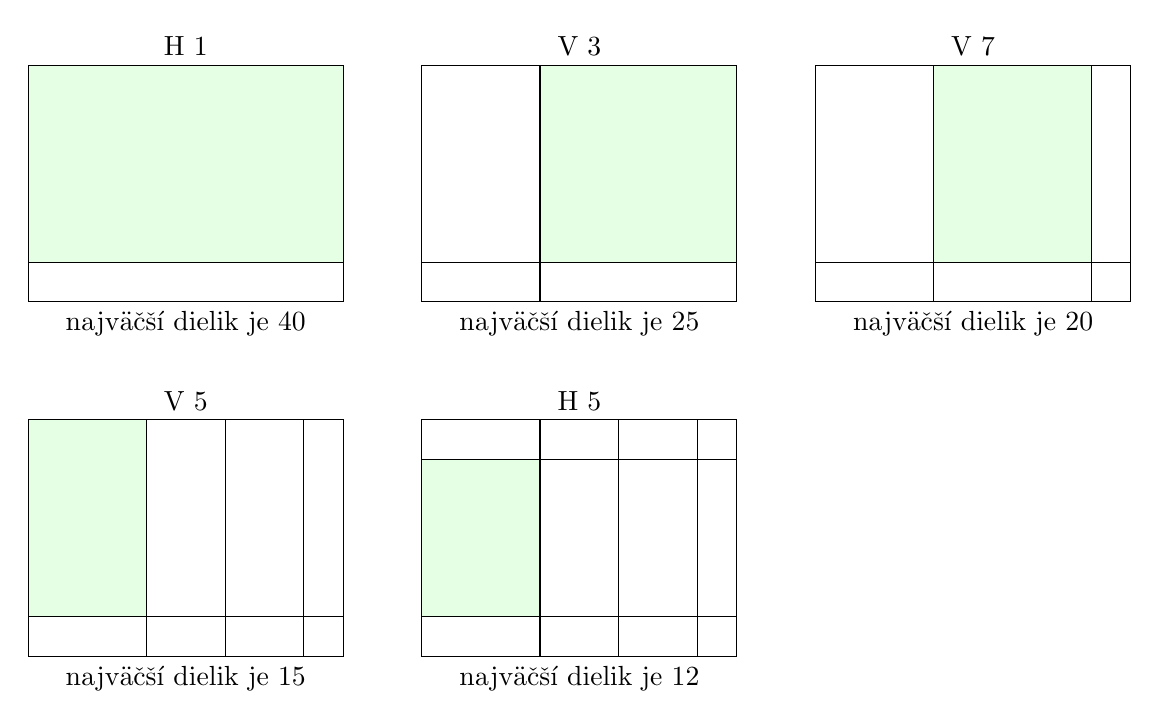
\begin{tikzpicture}[scale=0.5]
  \def\w{8}
  \def\h{6}
  \def\hlist{0}
  \def\vlist{0}
  \def\addH#1{\edef\hlist{\hlist,#1}}  
  \def\addV#1{\edef\vlist{\vlist,#1}}  
  \def\uloha(#1,#2)(#3,#4)#5#6{
    \filldraw[fill=green!10!white](#1,#2)rectangle(#3,#4);
    \draw (0,0) rectangle (\w,\h);
    \node [above] at (0.5*\w,\h) {\vb{#5}};
    \node [below] at (0.5*\w,0) {najväčší dielik je $#6$};
    \foreach\y in \hlist {\draw(0,\y)--(\w,\y);}
    \foreach\x in \vlist {\draw(\x,0)--(\x,\h);}
  }

    \addH1
    \uloha(0,1)(\w,\h){H 1}{40}

    \addV3
    \begin{scope}[shift={(10,0)}]
      \uloha(3,1)(\w,\h){V 3}{25}
    \end{scope}

    \addV7
    \begin{scope}[shift={(20,0)}]
      \uloha(3,1)(7,\h){V 7}{20}
    \end{scope}

    \addV5
    \begin{scope}[shift={(0,-9)}]
      \uloha(0,1)(3,\h){V 5}{15}
    \end{scope}

    \addH5
    \begin{scope}[shift={(10,-9)}]
      \uloha(0,1)(3,5){H 5}{12}
    \end{scope}
  \end{tikzpicture}}
\end{uloha}

\begin{uloha}
  V prvom riadku vstupu sú tri čísla $n$, $k$, $a$, ktoré predstavujú súčiastku, ktorú treba
  testovať. Je to rúrka dlhá $n$ a v nej je $k$ valčekov dĺžky $a$, ktoré sa nedotýkajú.
  Napr. pre $n=16$, $k=3$, $a=3$ niektoré správne súčiastky môžu vyzerať takto:

  
  \centerline{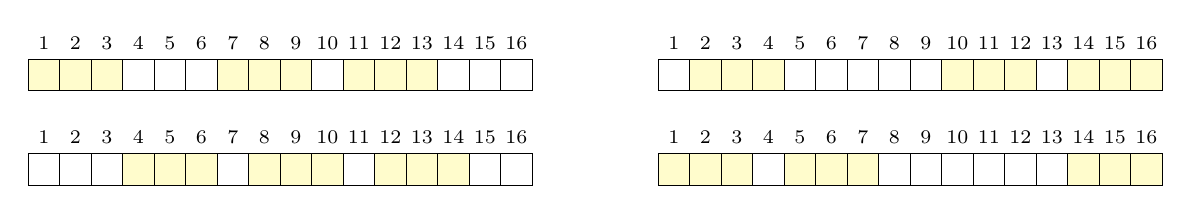
\begin{tikzpicture}[scale=0.4]
    \def\grd{%
    \foreach\x in {1,...,16} {
      \draw (\x-1,0) rectangle (\x,1);
      \node [above] at (\x-0.5,1) {{\scriptsize\roboto\x}};
    }
    }
    \def\rct#1{(#1,0) rectangle (#1+3,1)}

    \def\clr{yellow!20!white}
    \filldraw[\clr] \rct0 \rct6 \rct{10};
    \grd

    \begin{scope}[shift={(20,0)}]
      \filldraw[\clr] \rct1 \rct9 \rct{13};
    \grd
    \end{scope}

    \begin{scope}[shift={(0,-3)}]
      \filldraw[\clr] \rct3 \rct7 \rct{11};
    \grd
    \end{scope}

    \begin{scope}[shift={(20,-3)}]
      \filldraw[\clr] \rct0 \rct4 \rct{13};
    \grd
    \end{scope}
  \end{tikzpicture}}

  
  Ďalej je dané číslo $m$ a potom $m$ pozícií (číslovaných od 1), 
  na ktorých sa súčiastka testovala a zistilo sa,
  že na tej pozícii nie je valček. Napr. ak by sa testovali pozície $4,5,6,10,14$, súčiastka
  by mohla vyzerať ako vľavo hore. Keby ale na žiadnej z pozícií $4,5,6,10,14,1$ 
  valček nebol, tak je jasné,
  že súčiastka je chybná. Napíš program, ktorý prečíta jednotlivé testy a vypíše,
  po ktorom teste začne byť jasné, že súčiastka je chybná. 
\end{uloha}


Typy \prg!set! a \prg!map! sú síce naprogramované pomocou vyhľadávacích stromov, ale zámerom
je, že spôsob, akým sú naprogramované, je vecou kompilátora a teba ako programátora
to nemá čo zaujímať; máš len zaručené, že operácie vkladania, vyhľadávania a mazania
majú logaritmickú zložitosť. Preto ani nemáš v programe prístup priamo k uzlom stromu.
Niekedy by sa to ale hodilo. Nasledovný príklad ľahko vyriešiš, ak upravíš náš
AA strom \prg!Tree! tak, že každý uzol si bude navyše pamätať, 
koľko listov je v jeho podstrome.

\begin{uloha}
  Napíš program, ktorý vyhodnocuje postupnosť príkazov: \vb{pridaj x}, \vb{uber x}
  a \vb{? x}, kde \vb{x} je nejaké nezáporné celé číslo. Príkazy \vb{pridaj} a \vb{uber}
  pridávajú a uberajú čísla do/z množiny. 
  Pre každý príkaz \vb{? x} treba vypísať, koľko čísel 
  menších ako \vb{x} je momentálne v množine.
  Posledný príkaz je \vb{!}.
\end{uloha}

\begin{uloha}
  Napíš program, ktorý vyhodnocuje postupnosť príkazov: \vb{pridaj x}, \vb{uber x}
  a \vb{? x}, kde \vb{x} je nejaké nezáporné celé číslo. Príkazy \vb{pridaj} a \vb{uber}
  pridávajú a uberajú čísla do/z množiny. 
  Pre každý príkaz \vb{? x} treba vypísať $x$-té najmenšie číslo (brané od 0), ktoré
  sa v množine nenachádza.
  Posledný príkaz je \vb{!}.

  
  Napr. ak v množine sú čísla $\{2,3,6,8\}$ tak \vb{? 0} vráti \vb{0} (lebo $0$ nie
  je v množine), \vb{? 3} vráti \vb{5}
  lebo v množine nie sú čísla $0,1,4,5$ a \vb{? 5} vráti \vb{9}.
\end{uloha}

